\documentclass[12pt,a4paper,parskip]{scrartcl}
\usepackage[utf8]{inputenc}
\usepackage[T1]{fontenc}
\usepackage[ngerman]{babel}
\usepackage{lmodern}
\usepackage[babel,german=guillemets]{csquotes}
\usepackage[style=verbose-ibid,backend=bibtex8]{biblatex}
\bibliography{baclit110414}
\usepackage{amsmath}
\usepackage{amsfonts}
\usepackage{amssymb}
\usepackage{makeidx}
\usepackage{graphicx}
\usepackage{url}
\usepackage[locale=DE]{siunitx}%SI Einheiten etc.
\usepackage[german]{fancyref}%möglicherweise rausnehmen oder justieren
\usepackage{booktabs} %Tabellen Horizontale Linier dick darstellen
\usepackage{rotating}
\usepackage{lscape}
\usepackage{subfig}
\usepackage{here}
\usepackage{color}
\usepackage[left=3cm,right=3cm,top=2cm,bottom=2cm]{geometry}
\usepackage{mdwlist}
\begin{document}

\title{Messergebnisse}
\maketitle
Bitte beachten n vor Chargenbezeichnung steht für neue (also 2.) Versuchsreihe!
\newpage
\begin{figure}[H]
\centering
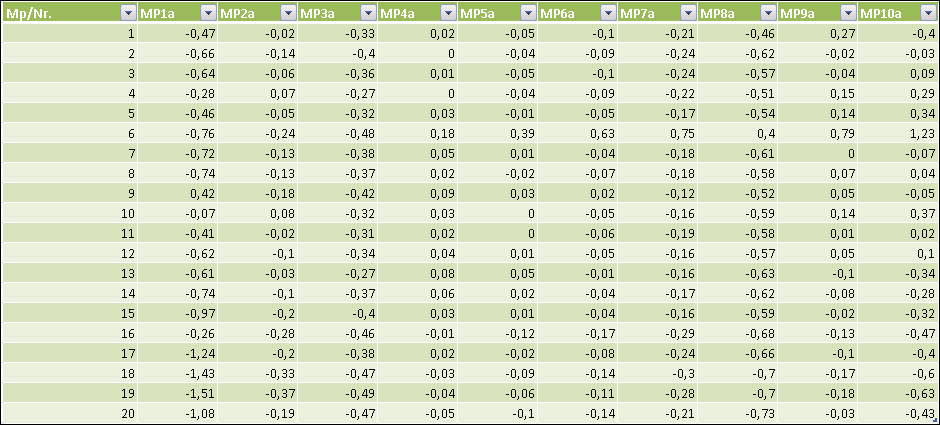
\includegraphics[width=1\textwidth]{BiegKontF13}
\caption{Streckbiegen, Kontur F13}
\end{figure}
\begin{figure}[H]
\centering
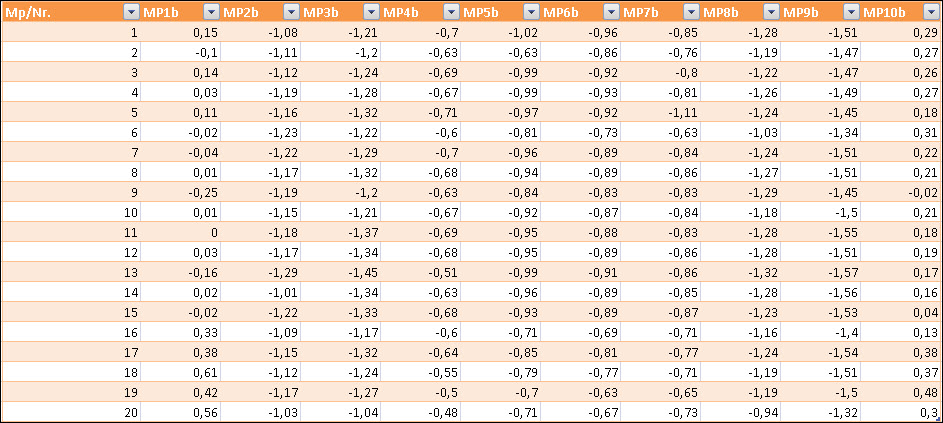
\includegraphics[width=1\textwidth]{BiegSpaltF13}
\caption{Streckbiegen, Spalt unten F13}
\end{figure}
\begin{figure}[H]
\centering
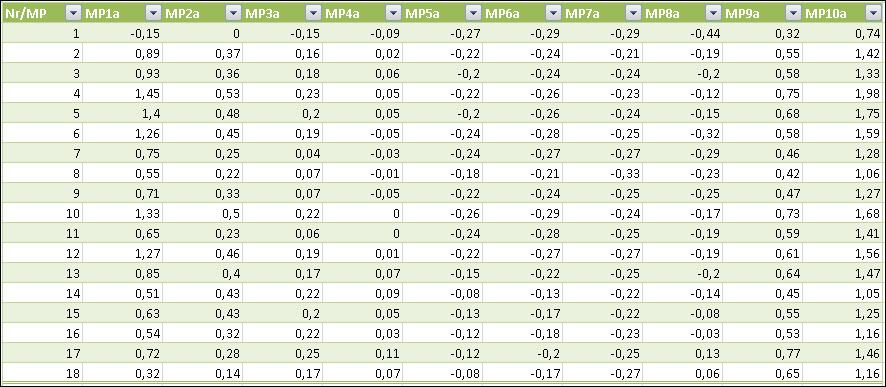
\includegraphics[width=1\textwidth]{BiegKontFxx}
\caption{Streckbiegen, Kontur Fxx}
\end{figure}
\begin{figure}[H]
\centering
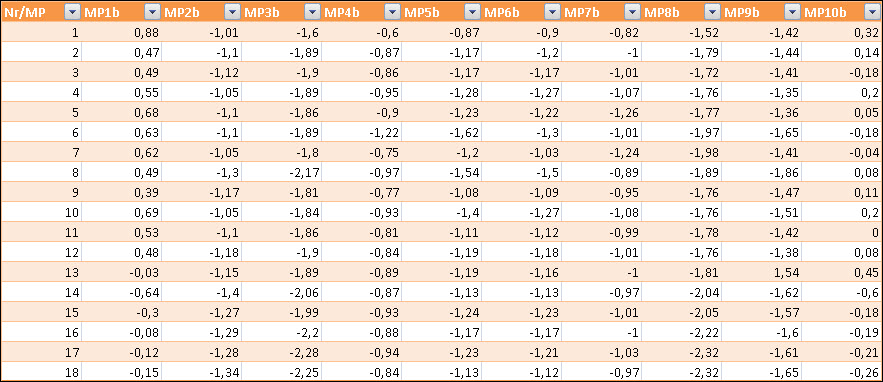
\includegraphics[width=1\textwidth]{BiegSpaltFxx}
\caption{Streckbiegen, Spalt unten Fxx}
\end{figure}
\begin{figure}[H]
\centering
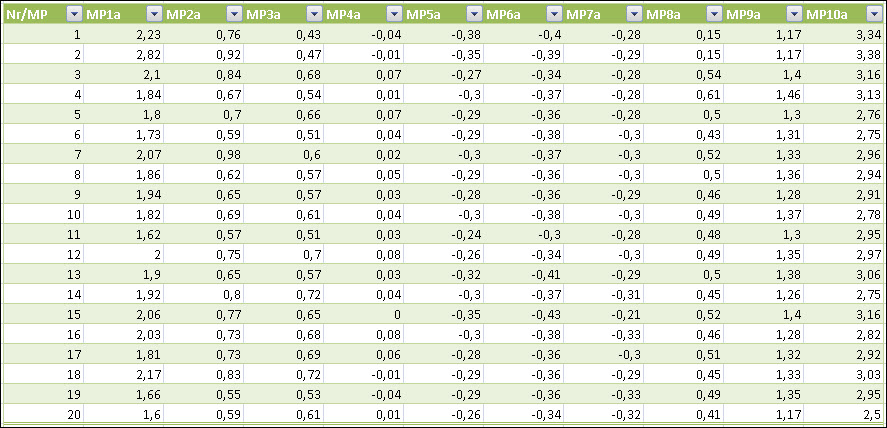
\includegraphics[width=1\textwidth]{BiegKontF17}
\caption{Streckbiegen, Kontur F17}
\end{figure}
\begin{figure}[H]
\centering
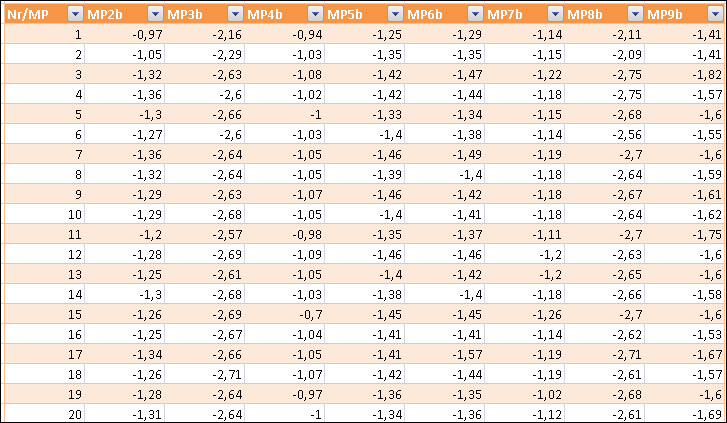
\includegraphics[width=1\textwidth]{BiegSpaltF17}
\caption{Streckbiegen, Spalt unten F17}
\end{figure}
\begin{figure}[H]
\centering
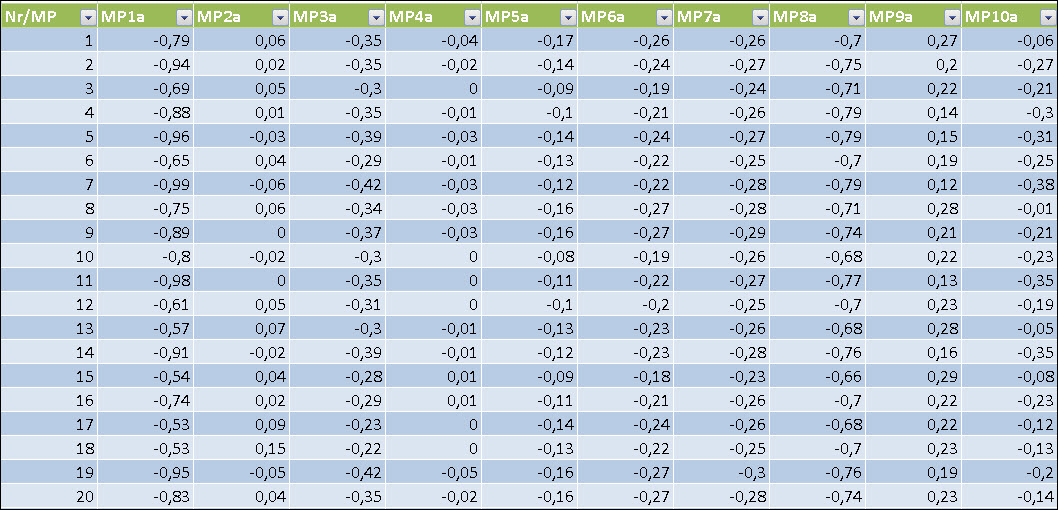
\includegraphics[width=1\textwidth]{BiegKontNF13}
\caption{Streckbiegen, Kontur nF13}
\end{figure}
\begin{figure}[H]
\centering
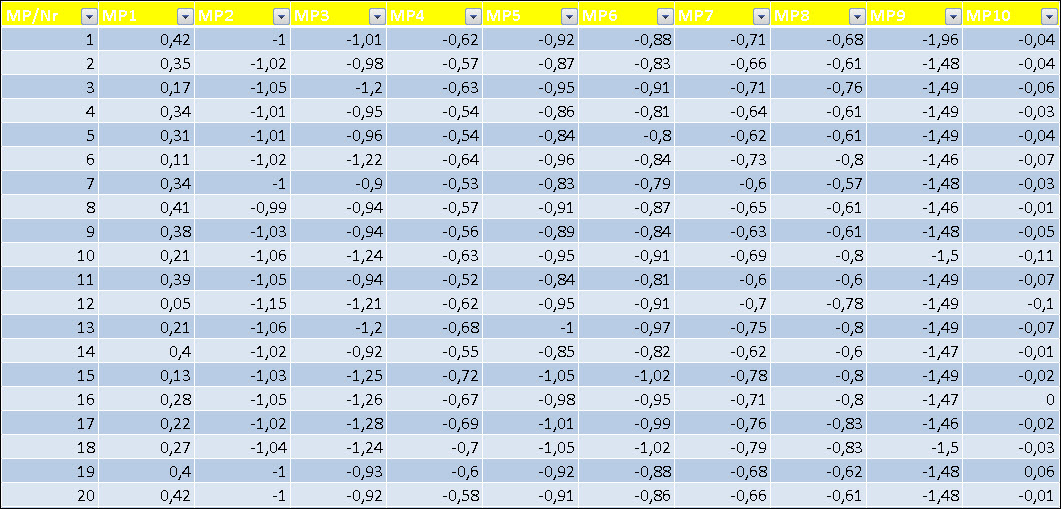
\includegraphics[width=1\textwidth]{BiegSpaltNF13}
\caption{Streckbiegen, Spalt unten nF13}
\end{figure}
\begin{figure}[H]
\centering
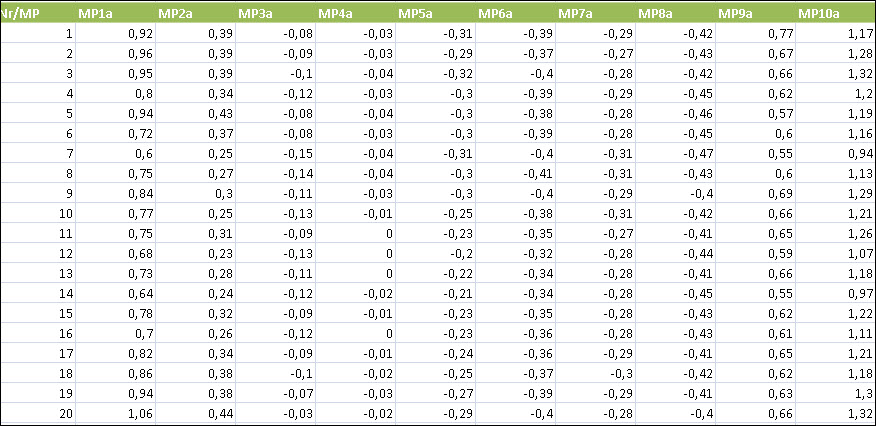
\includegraphics[width=1\textwidth]{BiegKontNFxx}
\caption{Streckbiegen, Kontur nFxx}
\end{figure}
\begin{figure}[H]
\centering
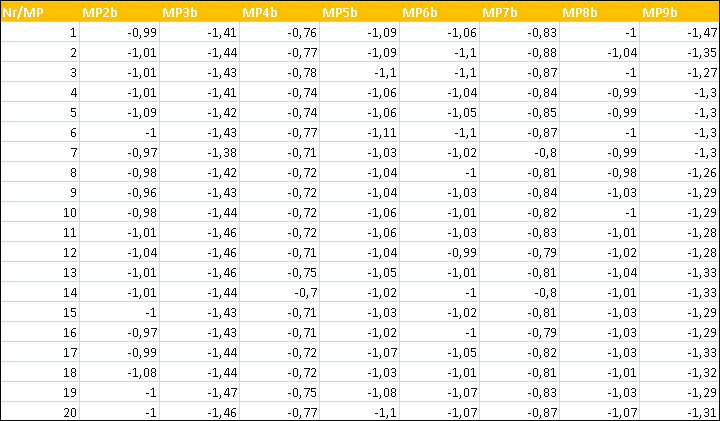
\includegraphics[width=1\textwidth]{BiegSpaltNFxx}
\caption{Streckbiegen, Spalt unten nFxx}
\end{figure}
\begin{figure}[H]
\centering
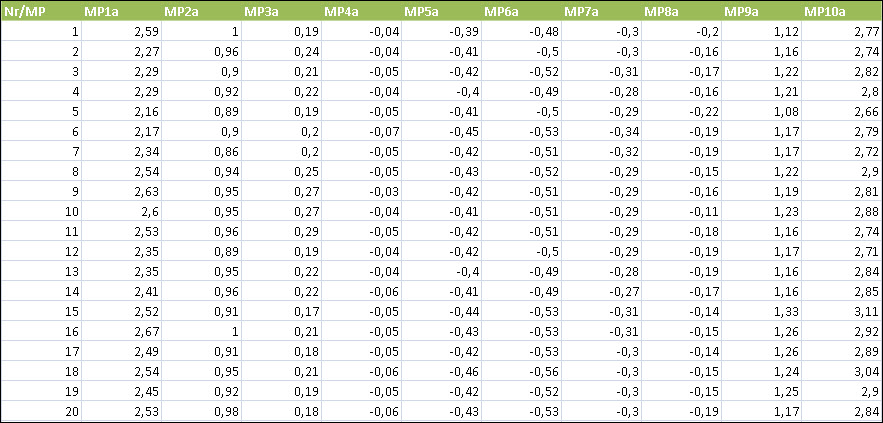
\includegraphics[width=1\textwidth]{BiegKontNF17}
\caption{Streckbiegen, Kontur nF17}
\end{figure}
\begin{figure}[H]
\centering
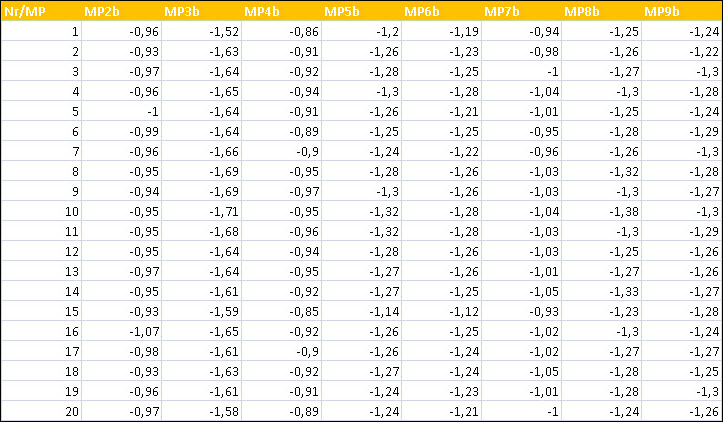
\includegraphics[width=1\textwidth]{BiegSpaltNF17}
\caption{Streckbiegen, Spalt unten nF17}
\end{figure}
\begin{figure}[H]
\centering
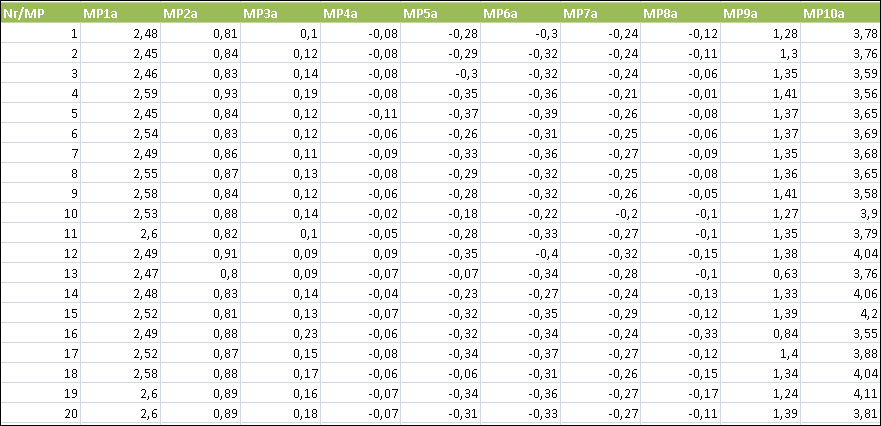
\includegraphics[width=1\textwidth]{BiegKontNF18}
\caption{Streckbiegen, Kontur nF18}
\end{figure}
\begin{figure}[H]
\centering
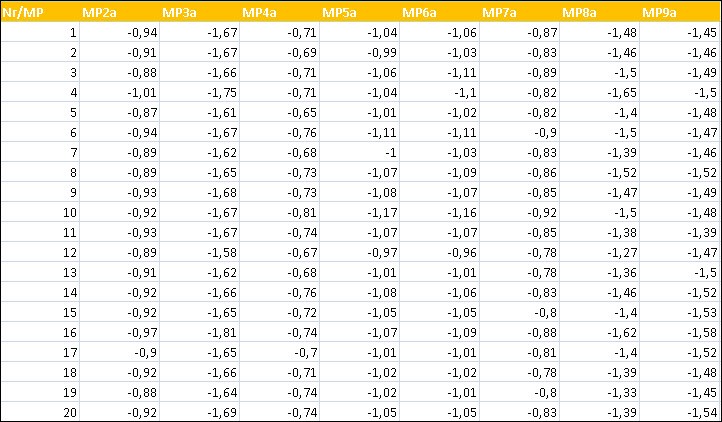
\includegraphics[width=1\textwidth]{BiegSpaltNF18}
\caption{Streckbiegen, Spalt unten nF18}
\end{figure}
\begin{figure}[H]
\centering
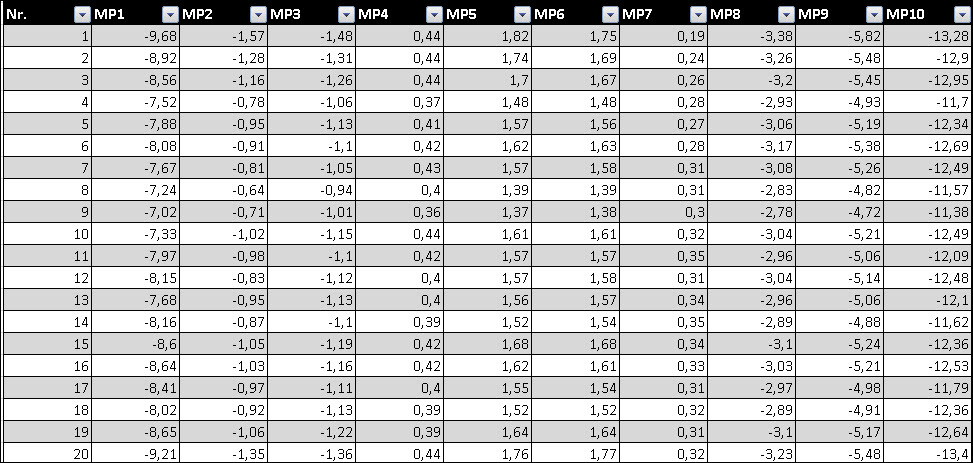
\includegraphics[width=1\textwidth]{BiegKontspaltinnenNF19}
\caption{Streckbiegen, Kontur nF19}
\end{figure}
\begin{figure}[H]
\centering
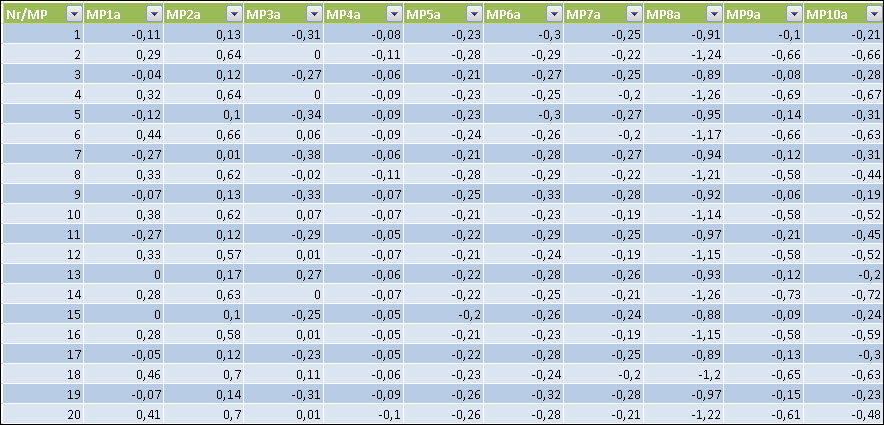
\includegraphics[width=1\textwidth]{FrasKontNF13}
\caption{Fräsen, Kontur nF13}
\end{figure}
\begin{figure}[H]
\centering
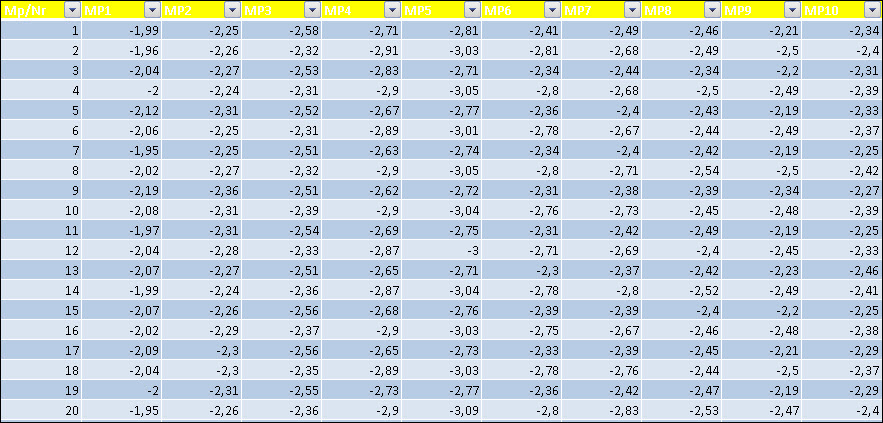
\includegraphics[width=1\textwidth]{FrasSpaltNF13}
\caption{Fräsen, Spalt unten nF13}
\end{figure}
\begin{figure}[H]
\centering
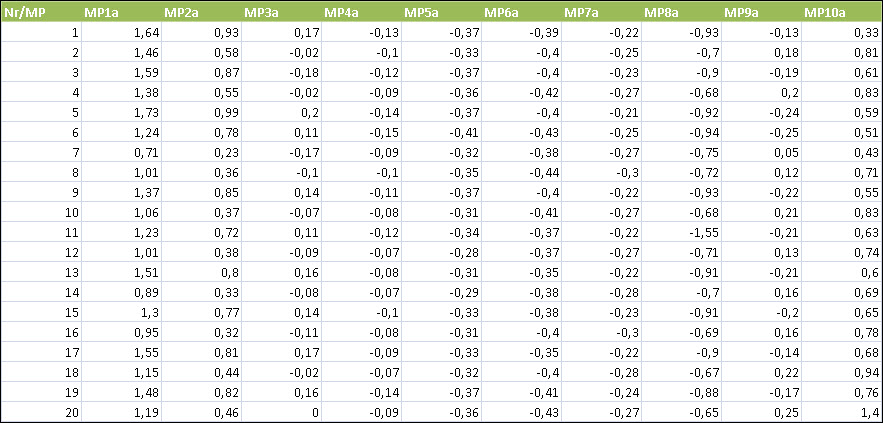
\includegraphics[width=1\textwidth]{FrasKontNFxx}
\caption{Fräsen, Kontur nFxx}
\end{figure}
\begin{figure}[H]
\centering
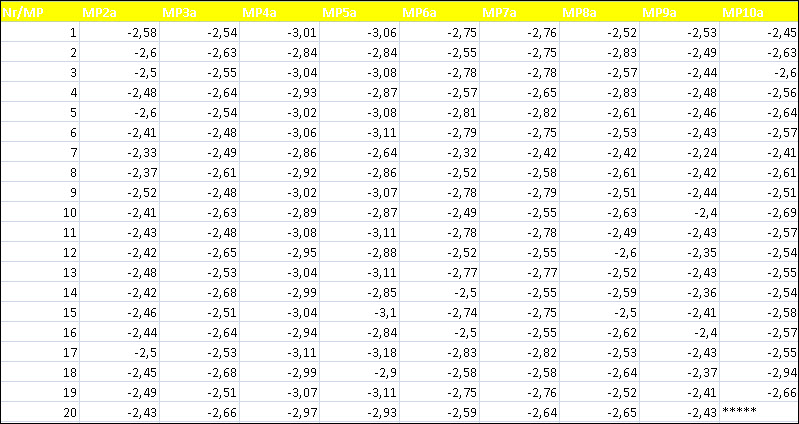
\includegraphics[width=1\textwidth]{FrasSpaltNFxx}
\caption{Fräsen, Spalt unten nFxx}
\end{figure}
\begin{figure}[H]
\centering
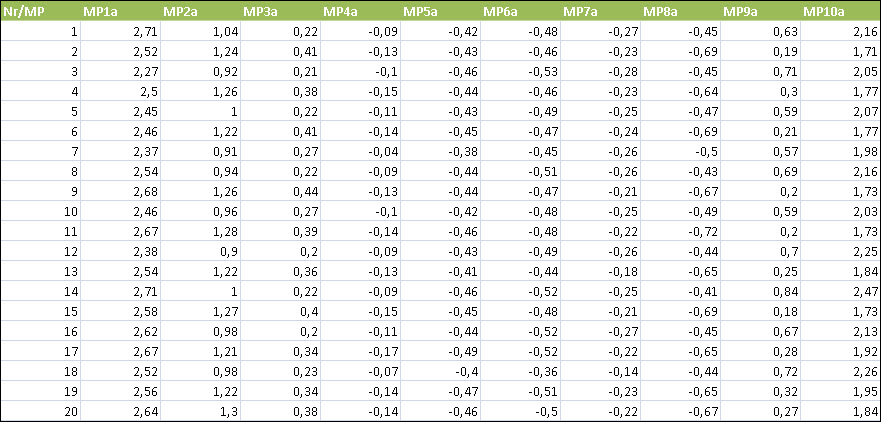
\includegraphics[width=1\textwidth]{FrasKontNF17}
\caption{Fräsen, Kontur nF17}
\end{figure}
\begin{figure}[H]
\centering
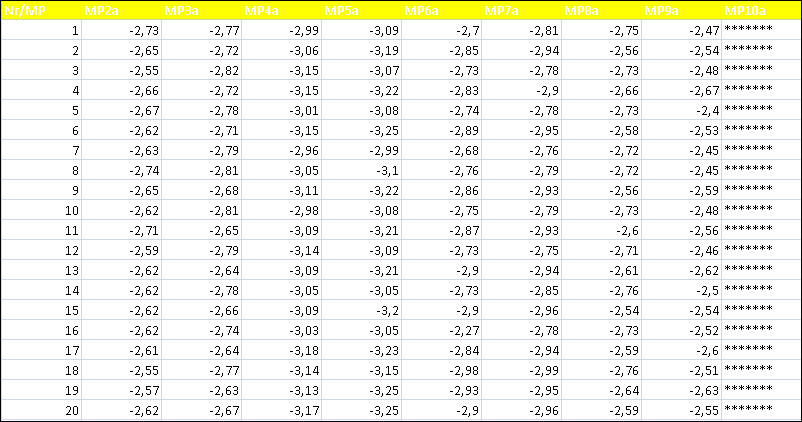
\includegraphics[width=1\textwidth]{FrasSpaltNF17}
\caption{Fräsen, Spalt unten nF17}
\end{figure}
\begin{figure}[H]
\centering
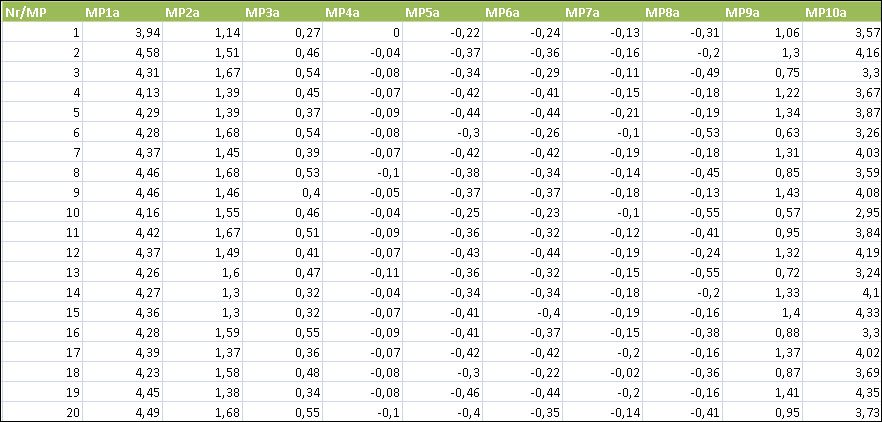
\includegraphics[width=1\textwidth]{FrasKontNF18}
\caption{Fräsen, Kontur nF18}
\end{figure}
\begin{figure}[H]
\centering
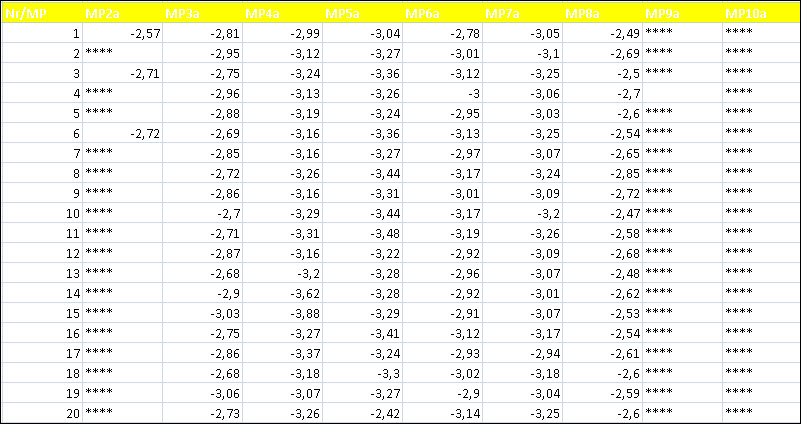
\includegraphics[width=1\textwidth]{FrasSpaltNF18}
\caption{Fräsen, Spalt unter nF18}
\end{figure}
\begin{figure}[H]
\centering
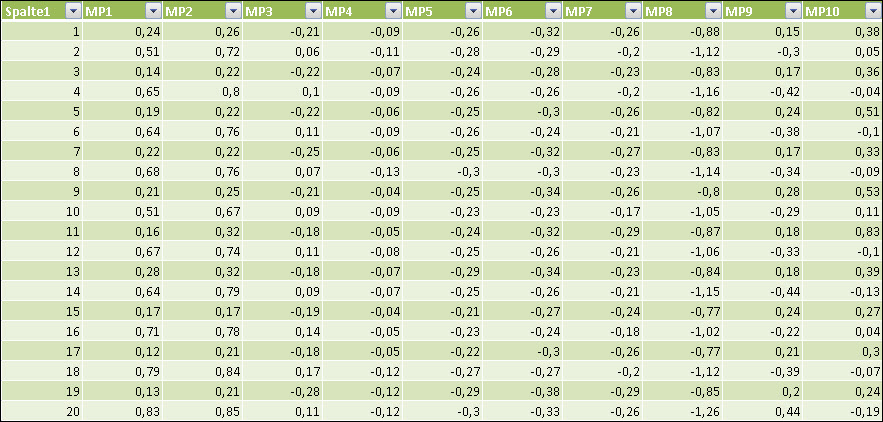
\includegraphics[width=1\textwidth]{PolierKontNF13}
\caption{Schleifen/Polieren, Kontur nF13}
\end{figure}
\begin{figure}[H]
\centering
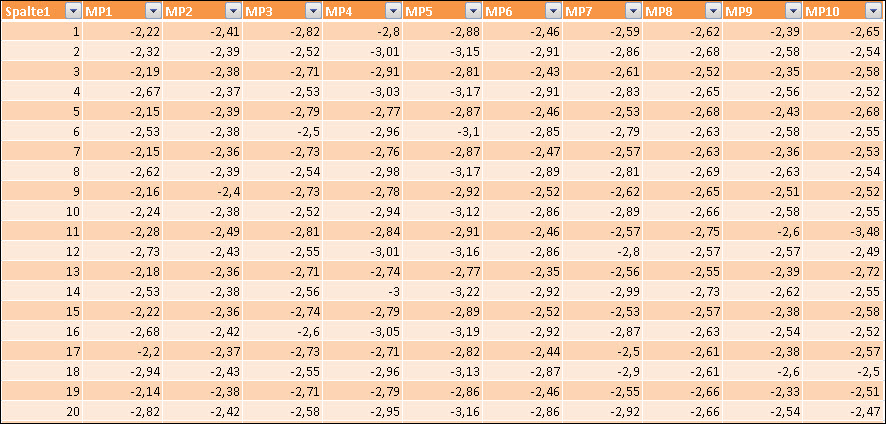
\includegraphics[width=1\textwidth]{PolierSpaltNF13}
\caption{Schleifen/Polieren, Spalt unten nF13}
\end{figure}
\begin{figure}[H]
\centering
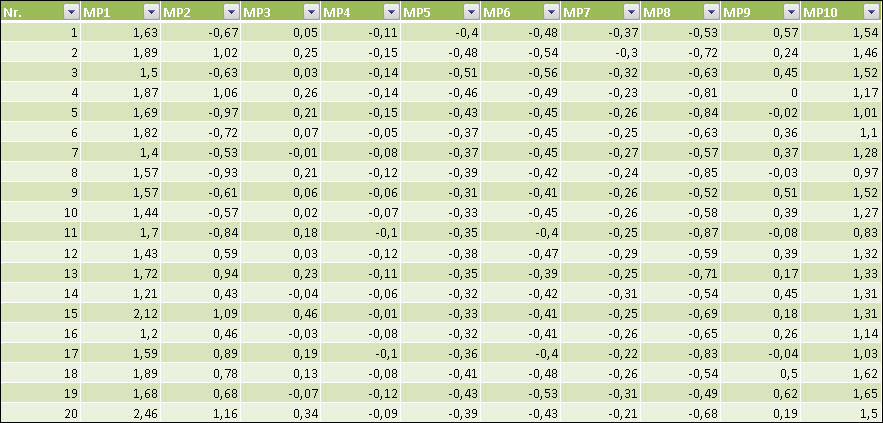
\includegraphics[width=1\textwidth]{PolierKontNFxx}
\caption{Schleifen/Polieren, Kontur nFxx}
\end{figure}
\begin{figure}[H]
\centering
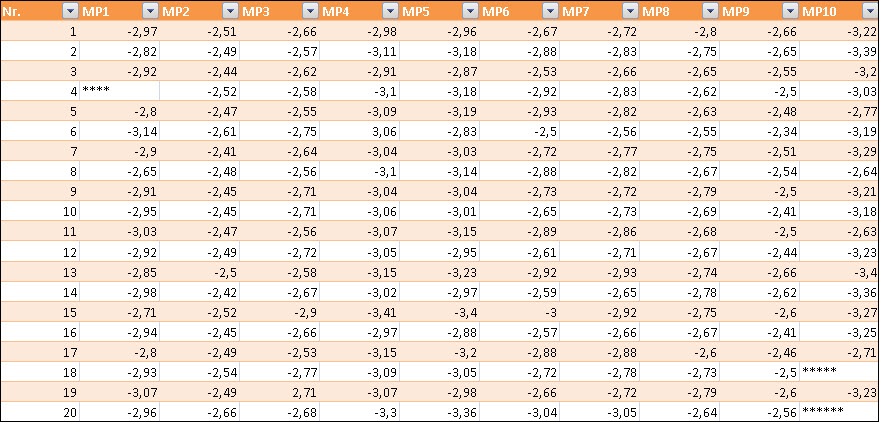
\includegraphics[width=1\textwidth]{PolierSpaltNFxx}
\caption{Schleifen/Polieren, Spalt unten nFxx}
\end{figure}
\begin{figure}[H]
\centering
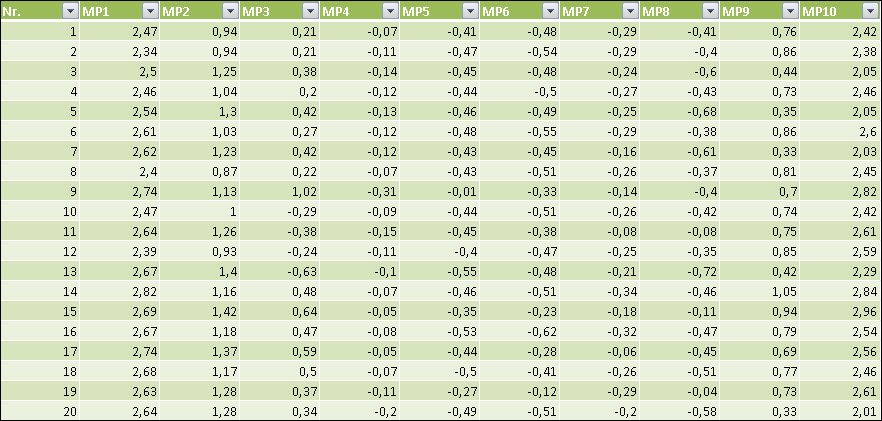
\includegraphics[width=1\textwidth]{PolierKontNF17}
\caption{Schleifen/Polieren, Kontur nF17}
\end{figure}
\begin{figure}[H]
\centering
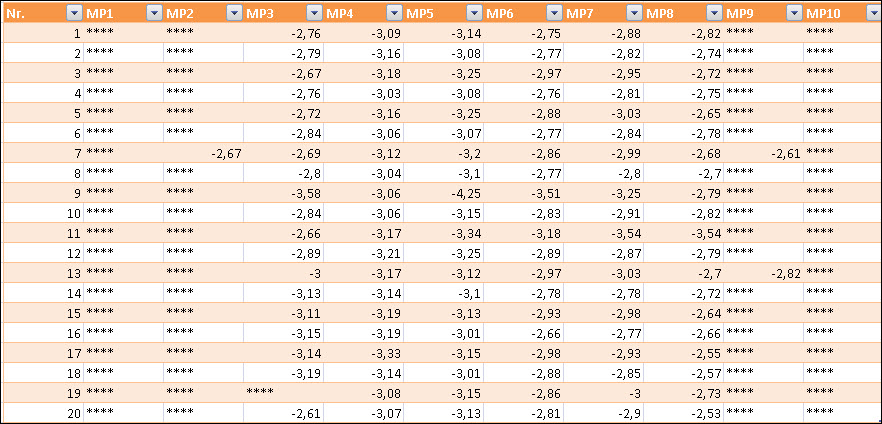
\includegraphics[width=1\textwidth]{PolierSpaltNF17}
\caption{Schleifen/Poliern, Spalt unten nF17}
\end{figure}
\begin{figure}[H]
\centering
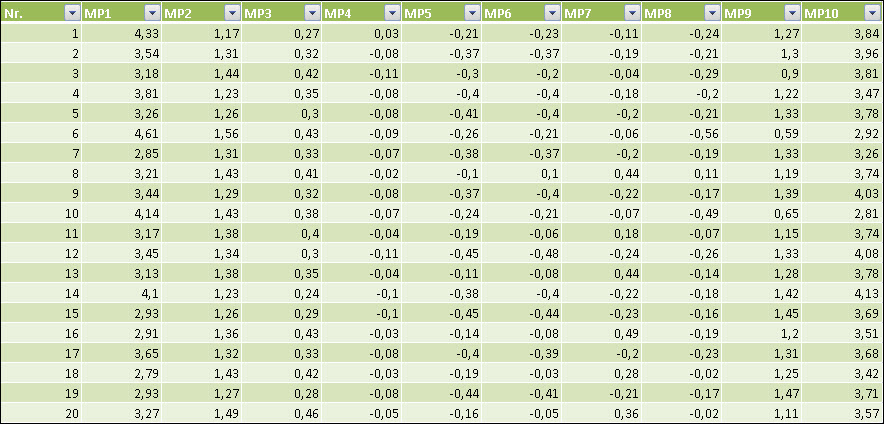
\includegraphics[width=1\textwidth]{PolierKontNF18}
\caption{Schleifen/Polieren, Kontur nF18}
\end{figure}


\end{document}  
